\chapter{DESAIN DAN IMPLEMENTASI}
\label{chap:desainimplementasi}

% Ubah bagian-bagian berikut dengan isi dari desain dan implementasi

Penelitian ini dilaksanakan sesuai dengan sistem berikut dengan implementasinya. Desain sistem merupakan konsep dari pembuatan dan perancangan infrastruktur dan kemudian diwujud kan dalam bentuk blok-blok alur yang harus dikerjakan. Pada bagian implementasi merupakan pelaksanaan teknis untuk setiap blok pada desain sistem.

\section{Deskripsi Sistem}
\label{sec:deskripsisistem}

Sistem pada tugas akhir ini merupakan implementasi dari salah satu disiplin ilmu \textit{Deep Learning} dan pengolahan citra yang berfungsi untuk mendeteksi adanya pejalan kaki yang berada di pinggir jalan, trotoar dan jalur penyebrangan. Selain pejalan kaki, deteksi juga dilakukan pada jalur penyebrangan atau \textit{zebracross} dengan tujuan untuk memberi informasi bahwa disekitar area tersebut terdapat banyak aktivitas pejalan kaki yang menyebrang jalan. Blok diagram metodologi sistem yang digunakan pada penelitian ini dapat dilihat pada Gambar \ref{fig:blok-diagram}.
\begin{figure}[ht]
	\centering
	
	% Ubah dengan nama file gambar dan ukuran yang akan digunakan
	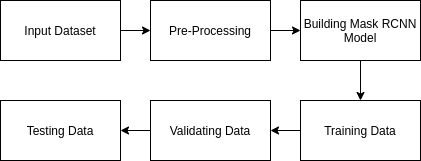
\includegraphics[scale=0.5]{gambar/blok-diagram.png}
	
	% Ubah dengan keterangan gambar yang diinginkan
	\caption{Blok Diagram Metodologi}
	\label{fig:blok-diagram}
\end{figure}   

\section{Implementasi Alat
\label{sec:implementasi alat}}

Alat diimplementasikan dengan \lipsum[1]

% Contoh pembuatan potongan kode
\begin{lstlisting}[
  language=C++,
  caption={Program halo dunia.},
  label={lst:halodunia}
]
#include <iostream>

int main() {
    std::cout << "Halo Dunia!";
    return 0;
}
\end{lstlisting}

\lipsum[2-3]

% Contoh input potongan kode dari file
\lstinputlisting[
  language=Python,
  caption={Program perhitungan bilangan prima.},
  label={lst:bilanganprima}
]{program/bilangan-prima.py}

\lipsum[4]
